% this file is drba_sw.tex
\section{Software}
\label{sec:software}
This section is all about the practical part of this work. At first, a brief reason why the software is implemented in C is given. Secondly, an accurate description is presented of how the software can be compiled and used for own demands.
After that, the software is tested on some randomly generated linear Codes. The number of degree compatible and all Groebner bases are presented and comparison of the operational time against Gfan \cite{gfan} is presented. \\
This software, called CIDGEL (Code Ideal degree compatible Groebner bases enumerating from Linear Codes), is a re-implementation of TiGERS \cite{tigers}. All features that are needed for the code ideals were added, also the adapted algorithms for computing degree compatible Groebner bases with reverse search and breath-first search were implemented.   
Additional features are explained in Section \ref{subsec:manual}.
The programming language of choice is C because it is fast and the capability to make own data structures are simple and sufficient enough.

\subsection{Data Structures}
\label{subsec:datastructure}
With the special attribute that code ideals only contains binomials and monomials and reduced Groebner bases have always the coefficent $1$, only the exponent vectors representing the monomials have to be stored.

\lstset{language=C, commentstyle=\color{green}, backgroundcolor=\color{white}, keywordstyle=\color{blue}, 
basicstyle = \ttfamily \color{black} \footnotesize , 
caption = { Data structure of binomials \cite{tigers} },frame = single, } 

\begin{lstlisting} 
typedef struct bin_tag *binomial;
struct bin_tag{
    int *exps1;
    int *exps2;
    int *E;
    int ff;
    int bf;
    binomial next;
};

\end{lstlisting}

The pointer \emph{exps1} stores the exponent vector of the first monomial and \emph{exps2} does it with the second monomial.
The integer \emph{ff} is a flag which shows if a binomial is a facet binomial or not and \emph{bf} tells if there is a monomial or binomial.
The pointer binomial next indicates that binomials are linked together like a linear list, which is necessary to describe ideals and Groebner bases.\\

The next code snippet shows the other important data structure. Again, it is a linked list like the binomials with the purpose to connect all reduced Groebner together, which is needed for the breath-first search.\\

The first four integers show off the identification number of the vertex of the edge graph, the number of facet binomials, number of binomials and the highest degree. Next is a pointer to the next generating set of the linked list.

The binomial \emph{cache\_edge} and the pointer \emph{cache\_vtx} stores the caching information in order not to recompute every facet binomial in the reverse search. 

\lstset{language=C, commentstyle=\color{green}, backgroundcolor=\color{white}, keywordstyle=\color{blue}, 
basicstyle = \ttfamily \color{black} \footnotesize , caption = {Data structure of generating sets },frame = single, } 
\begin{lstlisting} 
typedef struct gset_tag *gset;

/* Linked List of gset_tag which contiains the binomial and the
   caching informations*/
struct gset_tag{
    int id;
    int nfacets;
    int nelts;
    int deg;
    binomial bottom;
    binomial cache_edge;
    struct gset_tag *cache_vtx;
    struct gset_tag *next;
};

\end{lstlisting}

 


 


\subsection{Manual}
\label{subsec:manual}
This software was programmed and evaluated with Linux, so at first, it is needed to compile the software. The makefile is given and it only takes the console, moving to the direction where folder is and typing 'make'. \\
All inputs, outputs, options and flags are passed with the commandline arguments. At first it is useful to run the program with the purpose to print the help-message only with the command
\texttt{./cidgel -h}.

\lstset{basicstyle=\footnotesize, columns=fullflexible,showspaces=false,breakatwhitespace=true,caption = {Code Snippet of the help-message}} 
\begin{lstlisting} [showstringspaces=false,language=C,frame = single,]

static char *helpmsg[] = {
    "Function: Enumerate all or d.c Groebner bases of a code ideal I(C).",
    "          \n",
    "Options:\n",
    "    -h            print this message\n"
    "    -i (filename) set file name for input  [default: stdin]\n",
    "    -o (filename) set file name for output [default: stdout]\n",
    "    -m (filename) set file name for code-matching \n",
    "    -R            only compute root of tree \n",
    "    -r            compute all grobner bases [done by default]\n",
    "    -C            turn partial caching on   [done by default]\n",
    "    -c            turn partial caching off \n",
    "    -T            print edges of search tree \n",
    "    -t            do not print edges of search tree [assumed by default]\n",  
    "    -L            print vertices by giving initial ideals\n",
    "                     and printing facet biomials.\n",
    "    -l            print vertices as grobner bases   [done by default]\n",
    "    -F            Use only linear algebra when testing facets [default]\n",
    "    -f            use FLIPPABILITY test first when determining facets\n",
    "    -e            use exhaustive search instead of reverse search\n",
    "    -E            use reverse search                   [default]\n",
    "    -d            degree compatible Groebner bases only         \n",
    "    -n            do not print vertices or edges                \n",
    "    -p            calculate Groebner fans of punctured codes    \n",
    NULL
};

\end{lstlisting}

The listing above shows all options that are available. These flags can be passed in arbitrary order to the program. It is necessary to write a matrix and storing it into a file to give the program an input.

For example, the data has the name '\texttt{Example-input}', has the following content and is in the same folder as the compiled software.
\lstset{caption = {Example-input}}
\begin{lstlisting}[basicstyle=\fontfamily{courier}\selectfont]
M: { 6 10 2 :
1 0 0 0 0 0 0 0 1 1 
0 1 0 0 0 0 1 1 0 0 
0 0 1 0 0 0 1 1 1 1 
0 0 0 1 0 0 0 1 1 1 
0 0 0 0 1 0 1 0 0 0 
0 0 0 0 0 1 0 1 0 1 
}
\end{lstlisting}

This Matrix is a generator matrix for a binary $[10,6]$ code in essential standard form. 
The first number in the first row gives the code dimension, the second tells the length of the codeword and the last number indicates in which primary field the generator matrix shall be evaluated.\\

Now if the degree compatible Groebner bases of this generator  matrix without printing the Groebner basis shall be written in a outputfile called \texttt{Example-output}. Additionally the linear programming shall be leaved out, then the program call is: \texttt{./cidgel -i Example-input -o Example-output -d -n -f}.
The user do not has to specify an output file, the result will be printed in the console then.

\newpage

\lstset{caption = {Snippet of the example output}}
 \begin{lstlisting}[basicstyle=\fontfamily{courier}\selectfont,language={}] %
% starting GB:
F: 2
R: 10
G: {a-i*j, b-g*h, c-g*h*i*j, d-h*i*j, e-g, f-h*j,
	 g^2-1, h^2-1, i^2-1, j^2-1}

 Enumerating degree compatible Groebner bases
   using reverse search
   taking input from randomgenerator/10_6
   with partial caching
   using wall ideal pretest for facet checking

Number of Groebner bases found 216
Number of edges of state polytope 792
max caching depth      10
max facet binomials    18
min facet binomials    12
max binomials in GB    41
min binomials in GB    40
max degree             3
min degree             2
randomgenerator/10_6: Reverse Search,   Caching,  A-pretest,
time used (in seconds) 42.16
\end{lstlisting}
  



\subsection{Computational experience}
\label{subsec:compexp} 
In this section the difference between degree compatible Gröbner bases and all Gröbner bases from a linear Code are researched. Furthermore, the time for all Gröbner bases is compared against Gfan.
The linear codes were randomly generated.
\newpage
\begin{figure}[h]
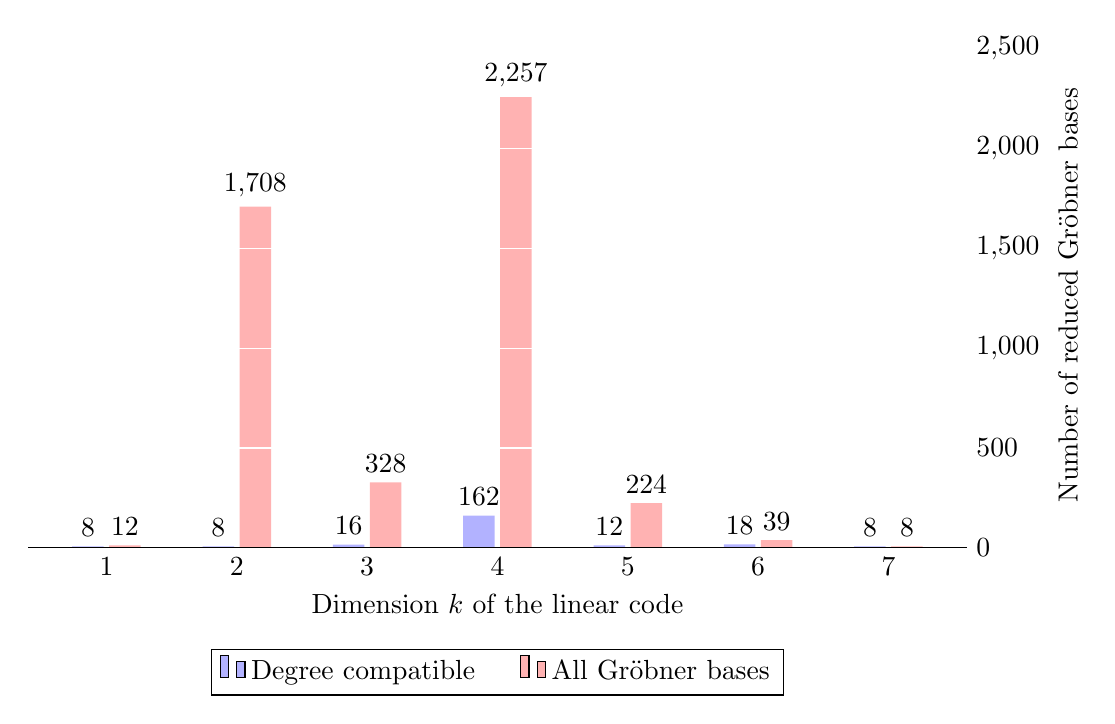
\begin{tikzpicture}
  \centering
  \begin{axis}[
        ybar, axis on top,
       % title={Example Text},
        height=8cm, width=13.5cm,
        bar width=0.4cm,
        ymajorgrids, tick align=inside,
        major grid style={draw=white},
        enlarge y limits={value=.1,upper},
        ymin=0, ymax=2300,
        axis x line*=bottom,
        axis y line*=right,
        y axis line style={opacity=0},
        tickwidth=0pt,
        enlarge x limits=true,
        legend style={
            at={(0.5,-0.2)},
            anchor=north,
            legend columns=-1,
            /tikz/every even column/.append style={column sep=0.5cm}
        },
        xlabel={Dimension $k$ of the linear code},
        ylabel={Number of reduced Gröbner bases},
        symbolic x coords={ 1,2,3,4,5,6,7},
       xtick=data,
       nodes near coords={
        \pgfmathprintnumber[precision=0]{\pgfplotspointmeta}
       }
    ]
    \addplot [draw=none, fill=blue!30] coordinates {
      (1,8)
      (2,8) 
      (3,16)
      (4,162) 
      (5,12) 
      (6,18)
      (7,8)};
      
   \addplot [draw=none,fill=red!30] coordinates {
      (1,12)
      (2,1708) 
      (3,328)
      (4,2257) 
      (5,224) 
      (6,39)
      (7,8)};
      

    \legend{Degree compatible,All Gröbner bases}
  \end{axis}
  \end{tikzpicture}
  \caption{Comparison between the numbers of degree compatible and all Gröbner bases }
  \label{fig:numbergb}
  \end{figure}
  
Figure \ref{fig:numbergb} shows a remarkable difference between all reduced Gröbner bases of a code ideal and the degree compatible. The length $n$ of the codeword is 8. The next table shows the computational time of the randomly generated codes.

 \begin{table}[h]
 \caption{Computataional time in seconds}
 \begin{tabular}{clll} % zentriert rest linksbündig
  Dimension $k$ & CIDGEL d.c. & CIDGEL & Gfan \\
  1  & 0.01  & 0.011  & 0.239  \\
  2  & 0.206 & 10.198 & 38.127 \\
  3  & 0.08  & 0.688  & 6.32 \\
  4  & 7.743 & 25.86  & 47.748 \\
  5  & 0.19  & 0.608  & 3.588  \\
  6  & 0.029 & 0.039  & 0.553\\
  7  & 0.009 & 0.009  & 0.116 \\
 \end{tabular}
 \label{tab:meinetabelle}
 \end{table}
 
 The table shows that the software CIDGEL can be way faster than Gfan for computing all the reduced Gröbner bases of a code ideal. The reason is the special binomial structure of the code ideals and the fast algorithms that can be linked with. Gfan is a software for Gröbner bases with more general structure.
 Even though the amount of all Gröbner bases are much more than the degree compatible Gröbner bases, the computational time does hold proportionally to the amount.
 The computational time depends most on the computation of facets, see page \pageref{facets}. The degree compatible Gröbner bases mostly have more binomials than all other Gröbner bases, that is why the computational time for a code ideal with a few Gröbner bases will last longer than for a code ideal with many Gröbner bases with low cardinality. \\
 
 For linear codes with the length more than 9 the computation took more than 10 hours for the complete Gröbner fan. The reason is that the amount of reduced Gröbner bases and the cardinality of each basis will be greater if the codewords will be longer. Nevertheless, the computation of the degree compatible Gröbner fan is useful for a certain length.\\
 
 In some cases the amount of the degree compatible and all Gröbner bases can enormously. A randomly generated $[9,2]$ code had 8 degree compatible Gröbner bases and overall 295.863 Gröbner bases. 
 
    

%TODO: EXTREMBEISPIEL ZEIGEN UND VLLT SAGEN WARUM NICHT FÜR GRÖSSERE BASEN 



\subsection{Documentation and electronic availability}
\label{subsec:docu}
A HTML-based documentation of the software is created with the help of doxygen.$[doxygen]$

\newpage

